\subsubsection{Rotação de Pontos no Plano Cartesiano}

Nesta seção, será vista a rotação de pontos, uma aplicação direta das fórmulas de adição de arcos vistas até então.

\begin{definition}
Considere o ponto $A = (x, y) \in \reais^2$ e chame de $\alpha$ o ângulo
formado pelo segmento $OA$ com o eixo positivo de $x$. A função
$T_{\theta} : \reais^2 \to \reais^2$  tal que
$$T_{\theta}\paren{x, y} = \paren{x\cdot \cos \theta - y\cdot \sen \theta, x\cdot \sen \theta + y\cdot \cos
\theta}$$ é a rotação de ângulo $\theta$ do ponto $A = (x,y)$ em
torno da origem. O esquema é ilustrado na Imagem~\ref{img:funcao-rotacao}.
%
\begin{figure}[H]
\centering
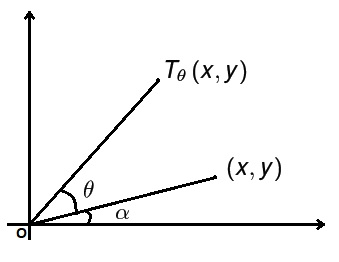
\includegraphics[scale=0.7]{\imgdirfromsection/rotacao.jpg}
\caption{Função de rotação $T_{\theta}$.}
\label{img:funcao-rotacao}
\end{figure}
\end{definition}

\begin{remark}
    Note que $x\cos \theta - y\sen\theta = \cos\alpha\cos\theta - \sen\alpha\sen\theta = \cos(\alpha+\theta)$ e que 
    $x \sen \theta + y\cdot \cos \theta = \cos\theta \cdot \sen\theta + \sen\alpha \cdot \cos\theta = \sen(\alpha+\theta)$, 
    ou seja, a rotação de pontos é, de fato, uma aplicação direta das identidades da Proposição~\ref{prop:seno-e-cosseno-da-soma}.
\end{remark}

\begin{onlineact}
    \khan{https://pt.khanacademy.org/math/trigonometry/trig-equations-and-identities/intro-to-trig-angle-addition-identities/e/trig_addition_identities}
    {Uso das Identidades Trigonométricas de Soma de Ângulos}.
\end{onlineact}

\begin{onlineact}
    \khan{https://pt.khanacademy.org/math/trigonometry/trig-equations-and-identities/using-trig-identities/e/applying-angle-addition-formulas}
    {Calcule Valores Trigonométricos a Partir de Identidades de Soma de Ângulos}.
\end{onlineact}